\documentclass[a4paper, 14pt]{extarticle}

% Поля
%--------------------------------------
\usepackage{geometry}
\geometry{a4paper,tmargin=2cm,bmargin=2cm,lmargin=3cm,rmargin=1cm}
%--------------------------------------


%Russian-specific packages
%--------------------------------------
\usepackage[T2A]{fontenc}
\usepackage[utf8]{inputenc} 
\usepackage[english, main=russian]{babel}
%--------------------------------------

\usepackage{textcomp}

% Красная строка
%--------------------------------------
\usepackage{indentfirst}               
%--------------------------------------             


%Graphics
%--------------------------------------
\usepackage{graphicx}
\graphicspath{ {./images/} }
\usepackage{wrapfig}
%--------------------------------------

% Полуторный интервал
%--------------------------------------
\linespread{1.3}                    
%--------------------------------------

%Выравнивание и переносы
%--------------------------------------
% Избавляемся от переполнений
\sloppy
% Запрещаем разрыв страницы после первой строки абзаца
\clubpenalty=10000
% Запрещаем разрыв страницы после последней строки абзаца
\widowpenalty=10000
%--------------------------------------

%Списки
\usepackage{enumitem}

%Подписи
\usepackage{caption} 

%Гиперссылки
\usepackage{hyperref}

\hypersetup {
	unicode=true
}

%Рисунки
%--------------------------------------
\DeclareCaptionLabelSeparator*{emdash}{~--- }
\captionsetup[figure]{labelsep=emdash,font=onehalfspacing,position=bottom}
%--------------------------------------

\usepackage{tempora}

%Листинги
%--------------------------------------
\usepackage{listings}
\lstset{
  basicstyle=\ttfamily\footnotesize, 
  %basicstyle=\footnotesize\AnkaCoder,        % the size of the fonts that are used for the code
  breakatwhitespace=false,         % sets if automatic breaks shoulbd only happen at whitespace
  breaklines=true,                 % sets automatic line breaking
  captionpos=t,                    % sets the caption-position to bottom
  inputencoding=utf8,
  frame=single,                    % adds a frame around the code
  keepspaces=true,                 % keeps spaces in text, useful for keeping indentation of code (possibly needs columns=flexible)
  keywordstyle=\bf,       % keyword style
  numbers=left,                    % where to put the line-numbers; possible values are (none, left, right)
  numbersep=5pt,                   % how far the line-numbers are from the code
  xleftmargin=25pt,
  xrightmargin=25pt,
  showspaces=false,                % show spaces everywhere adding particular underscores; it overrides 'showstringspaces'
  showstringspaces=false,          % underline spaces within strings only
  showtabs=false,                  % show tabs within strings adding particular underscores
  stepnumber=1,                    % the step between two line-numbers. If it's 1, each line will be numbered
  tabsize=2,                       % sets default tabsize to 8 spaces
  title=\lstname                   % show the filename of files included with \lstinputlisting; also try caption instead of title
}
%--------------------------------------

%%% Математические пакеты %%%
%--------------------------------------
\usepackage{amsthm,amsfonts,amsmath,amssymb,amscd}  % Математические дополнения от AMS
\usepackage{mathtools}                              % Добавляет окружение multlined
\usepackage[perpage]{footmisc}
%--------------------------------------

%--------------------------------------
%			НАЧАЛО ДОКУМЕНТА
%--------------------------------------

\begin{document}

%--------------------------------------
%			ТИТУЛЬНЫЙ ЛИСТ
%--------------------------------------
\begin{titlepage}
\thispagestyle{empty}
\newpage


%Шапка титульного листа
%--------------------------------------
\vspace*{-60pt}
\hspace{-65pt}
\begin{minipage}{0.3\textwidth}
\hspace*{-20pt}\centering

\includegraphics[width=\textwidth]{emblem}
\end{minipage}
\begin{minipage}{0.67\textwidth}\small \textbf{
\vspace*{-0.7ex}
\hspace*{-6pt}\centerline{Министерство науки и высшего образования Российской Федерации}
\vspace*{-0.7ex}
\centerline{Федеральное государственное бюджетное образовательное учреждение }
\vspace*{-0.7ex}
\centerline{высшего образования}
\vspace*{-0.7ex}
\centerline{<<Московский государственный технический университет}
\vspace*{-0.7ex}
\centerline{имени Н.Э. Баумана}
\vspace*{-0.7ex}
\centerline{(национальный исследовательский университет)>>}
\vspace*{-0.7ex}
\centerline{(МГТУ им. Н.Э. Баумана)}}
\end{minipage}
%--------------------------------------

%Полосы
%--------------------------------------
\vspace{-25pt}
\hspace{-35pt}\rule{\textwidth}{2.3pt}

\vspace*{-20.3pt}
\hspace{-35pt}\rule{\textwidth}{0.4pt}
%--------------------------------------

\vspace{1.5ex}
\hspace{-35pt} \noindent \small ФАКУЛЬТЕТ\hspace{80pt} <<Информатика и системы управления>>

\vspace*{-16pt}
\hspace{47pt}\rule{0.83\textwidth}{0.4pt}

\vspace{0.5ex}
\hspace{-35pt} \noindent \small КАФЕДРА\hspace{50pt} <<Теоретическая информатика и компьютерные технологии>>

\vspace*{-16pt}
\hspace{30pt}\rule{0.866\textwidth}{0.4pt}
  
\vspace{11em}

\begin{center}
\Large {\bf Лабораторная работа № 6} \\
\large {\bf по курсу <<Численные методы линейной алгебры>>} \\
\large <<Изучение скорости сходимости однопараметрического метода>>
\end{center}\normalsize

\vspace{8em}


\begin{flushright}
  {Студентка группы ИУ9-72Б Самохвалова П. С. \hspace*{15pt}\\
  \vspace{2ex}
  Преподаватель Посевин Д. П.\hspace*{15pt}}
\end{flushright}

\bigskip

\vfill
 

\begin{center}
\textsl{Москва 2023}
\end{center}
\end{titlepage}
%--------------------------------------
%		КОНЕЦ ТИТУЛЬНОГО ЛИСТА
%--------------------------------------

\renewcommand{\ttdefault}{pcr}

\setlength{\tabcolsep}{3pt}
\newpage
\setcounter{page}{2}

\section{Цель работы}\label{Sect::goal}

Изучить зависимость скорости сходимости однопараметрического метода в зависимости от значения $\tau$.

\section{Задание}\label{Sect::task}

\begin{itemize}
    \item Реализовать однопараметрический метод для положительной симметричной матрицы произвольного размера N x N.
    \item Вычислить спектр матрицы A методом Крылова или Данилевского, которые были реализованы ранее, и получить минимальное и максимальное значение спектра $\lambda_{min}$ и $\lambda_{max}$. После чего вычислить $\tau_{opt}$ = 2 / ($\lambda_{min}$ + $\lambda_{max}$).
    \item Построить график зависимости количества итераций n решения уравнения A·x = f однопараметрическим методом в зависимости от значения $\tau$ лежащего в пределах от 0 до 2 / $\lambda_{max}$. Определить $\tau_{opt}$ из графика и сравнить с теоретическим значением полученным в пункте 2.
    \item Для каждого эксперимента пункта 3 вывести условие сходимости посчитанное по формуле:
          \begin{figure}[!htb]
              \centering
              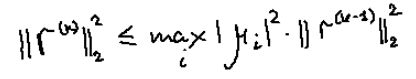
\includegraphics[width=0.8\textwidth]{img4}
          \label{fig:img4}
          \end{figure}

          Решение x* системы уравнения Ax = f для оценки неравенства приведенного выше можно получить путем решения Ax = f методом Гаусса. Другими словами, требуется убедиться в том, что выполняются условия теоремы о сходимости однопараметрического метода. Обязательно, дополнительно проверить и показать, что для каждого k модуль максимального значения $\mu_i$ меньше 1.
\end{itemize}

\section{Практическая реализация}\label{Sect::code}

Исходный код программы представлен в листинге~\ref{lst:code1}.

\begin{lstlisting}[language={python},caption={Однопараметрический метод},label={lst:code1}]
from num_methods import *

n = 5
a = generate_symm_matrix(n, 1, 10)
a = increase_diagonal_elements_to_diagonal_predominance(a)
x_true = [i for i in range(1, n + 1)]
f = mult_matr_vec(a, x_true)

d, b = danilevsky_method(a)
p1 = d[0][:]
g1 = gershgorin_rounds(a)
ls = div_half_method(g1[0], g1[1], func(p1))

l_min = min(ls)
l_max = max(ls)
t_opt = 2 / (l_min + l_max)

print("t optimal")
print(t_opt)
print()

eps = 0.0001

ks = []
ts = []

t_start = 0.0001

t = t_start

t_opt_graphic = t
k_min = 0

while t < 2 / l_max:
    k = 0
    x_old = [0] * n
    p = sub_matr_matr(generate_unit_matr(n), mult_matr_num(t, a))
    g = mult_vec_num(t, f)

    max_m = 0
    for i in range(len(ls)):
        m = 1 - t * ls[i]
        if abs(m) > max_m:
            max_m = abs(m)
    if max_m >= 1:
        print("max_m >= 1")

    while True:
        x = sum_vec(mult_matr_vec(p, x_old), g)
        if norm_vec(sub_vec(x, x_old)) < eps:
            break
        if round(norm_vec_sq(sub_vec(x_true, x)), 5) > round((max_m**2) * norm_vec_sq(sub_vec(x_true, x_old)), 5):
            print("Convergence condition is not satisfied")
        x_old = x[:]
        k += 1
    if t == t_start:
        k_min = k
        t_opt_graphic = t
    elif k <= k_min:
        k_min = k
        t_opt_graphic = t
    ts.append(t)
    ks.append(k)
    t += 0.0001

print("t optimal graphic")
print(t_opt_graphic)

plt.xlabel('t')
plt.ylabel('k')
plt.grid()
plt.plot(ts, ks)
plt.show()

\end{lstlisting}

\section{Результаты}\label{Sect::res}

Результаты работы программы представлены на рисунках~\ref{fig:img1}~--~\ref{fig:img3}.

\begin{figure}[!htb]
	\centering
	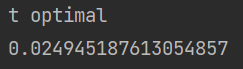
\includegraphics[width=0.8\textwidth]{img1}
\caption{$\tau$ оптимальное, полученное аналитически}
\label{fig:img1}
\end{figure}

\begin{figure}[!htb]
	\centering
	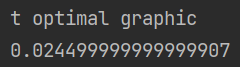
\includegraphics[width=0.8\textwidth]{img2}
\caption{$\tau$ оптимальное, полученное из графика}
\label{fig:img2}
\end{figure}

\begin{figure}[!htb]
	\centering
	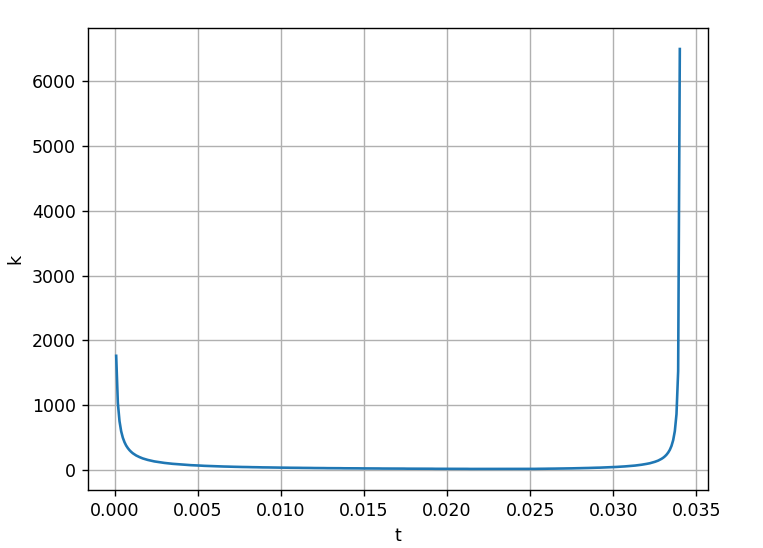
\includegraphics[width=0.8\textwidth]{img3}
\caption{График}
\label{fig:img3}
\end{figure}

\section{Выводы}\label{Sect::conclusion}

В результате выполнения лабораторной работы была изучена зависимость скорости сходимости однопараметрического метода в зависимости от значения $\tau$.
\end{document}
